\documentclass[12pt]{extarticle}
\usepackage[english]{babel}
\usepackage[utf8]{inputenc}
\usepackage{amsmath}
\usepackage{graphicx}
\usepackage[colorinlistoftodos]{todonotes}
\usepackage[hidelinks]{hyperref}
\usepackage{courier}
\usepackage{booktabs}
\usepackage[T1]{fontenc}
\usepackage{tabularx}
\usepackage[margin=0.5in]{geometry}
\usepackage{breakurl}
\fontencoding{T1}
\fontfamily{calibri}
\fontsize{12}{15}
\selectfont

\begin{document}
\begin{center}
\bf \Huge BoxIn\\
Developer Guide

\includegraphics[width=\textwidth]{BoxIn}
\end{center}

\pagebreak

\tableofcontents

\pagebreak

\section{Background}

BoxIn is a C++ based to-do list manager and this guide will help to understand how it works. BoxIn design adheres to the following coding standards

\subparagraph{SLAP}    
SLAP refers to Single Level Abstraction Principle. Code should be well abstracted so that each function only has one level of function calls. This helps to keep code from becoming convoluted by abstracting away the details of how a function is implemented

\subparagraph{Memory Management}
Coding in C++ requires efficient use of memory. Memory should be freed if its not in use any longer.

\subparagraph{Compatibility}
Code should be written such that is is cross platform and compatible with different compilers. Compiler specific code should be marked as such.

\subparagraph{Coding standard}
BoxIn code follows the coding standard listed out here: \href{https://docs.google.com/document/pub?id=1tJD2XQo3hUb0SZniswLqg0vkmccv7vGBV7\_1AhTYK04\&amp\&embedded=true}{C++ coding standards}.

\subparagraph{Namespaces}
All namespaces should be marked out to avoid confusion with the Boost library which is used in many parts of the code. For example, \texttt{std::string} rather than simply \texttt{string}\\
\newpage


\section{Anatomy}

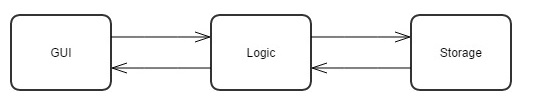
\includegraphics[width=\textwidth]{architecture}

BoxIn has 4 major components, the GUI, the Logic, the Storage and the Parser components. The components are divided in a way that follows two guiding principles. We also apply the Model View Controller pattern.

\subsection{Model View Controller pattern}
In BoxIn, the GUI component acts as both the View and the Controller. Users view all events through the GUI and the GUI is also responsible for taking care of all user interaction, including mouse clicks and information sent through the command line. More details are found in Section 3.
The Model in the system is the Event class. More details are found in Section 5.

\subsection{Separation of Concerns}
Each major component of the application handles it's own concerns. For example, the GUI or Storage components do not process any command line input, only the Logic and parsers do.

\subsection{Law of Demeter}
This law is particularly effected in the fact that the GUI and the Storage classes have no knowledge of each other - neither calls any functions of the other. Essentially, classes which do not have any direct relation with each other should not be calling each other.

\newpage
\section{GUI}
\includegraphics[width=\textwidth]{GUI_class_diagram}
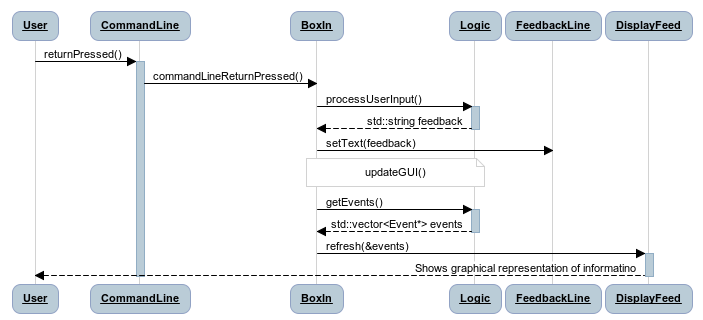
\includegraphics[width=\textwidth]{gui_sequence_diagram}

\newpage

The GUI component acts as both the controller and the view in the MVC pattern. The library used to is the Qt library. The documentation for the Qt library is available here: \href{http://qt-project.org/doc/}{http://qt-project.org/doc/}\\
The above diagrams give a graphical representation of how the \texttt{GUI} is designed in both the sequential calls on user actions and as a component.
The GUI is divided into 7 components, discussed below

\subsection{BoxIn (main window)}
The \texttt{BoxIn} class is the main window. All sub-components found in this window should also have this window as a parent window. This class inherits from \texttt{QWidget}. The \texttt{BoxIn} class mainly acts as a container for most of the GUI components\\
The above sequence diagram shows the generic flow of events within the GUI component everytime the user presses the return key\\
\subparagraph{Private attributes}
\begin{tabular}{l r}
Attribute type & Name\\
\hline
Ui::BoxInClass & ui\\
Logic & logic\\
QAction* & minimizeAction\\
QAction* & restoreAction\\
QAction* & quitAction\\
DigitalClock & clock\\
QLabel* & nameLabel\\
QLabel* & placeLabel\\
QLabel* & startLabel\\
QLabel* & idxLabel\\
QSystemTrayIcon* & trayIcon\\
QMenu* & trayIconMenu\\
DisplayFeed* & displayFeedIdx\\
QLineEdit* & commandLine\\
\end{tabular}
\subparagraph{Public methods}
\begin{tabular}{l r}
Return type & Method\\
\hline
void & displayFeedback(QString feedback)\\
void & clearCommandLine()\\
QString & readCommandLine()\\
void & setVisible(bool visible)\\
void & updateGUI()\\
void & createComponents()\\
void & setComponentSizes()\\
void & setComponentColors()\\
void & linkEvents()\\
void & createTrayIcon()\\
void & createActions()\\
void & iconActivatd()\\
void & changeEvent(QEvent *event);\\
\end{tabular}\\

\subparagraph{Key API}
The following are the key methods that deal with functionality of the GUI\\
\begin{tabular}{p{6cm} p{12cm}}
Method & Description\\
\hline
returnPressed() & This signal is by the Qt framework whenever the user presses return with the command line in focus\\
linkEvents() & This method is a setup method linking all the relevant signals to the respective slots for processing\\
commandLineReturnPressed() & The slot connected to the returnPressed() signal mentioned above. This starts the chain of events which result in event processing, by reading the line and sending it to the Logic component\\
readCommandLine() & Returns the string held by the command line. Called exclusively by commandLineReturnPressed()\\
clearCommandLine() & Removes any text in the commandLine. Also called exclusively by commandLineReturnPressed()\\
displayFeedback(QString feedback) & Calls setText() on the FeedbackLine to display feedback\\
\end{tabular}

\subparagraph{Application icon}
The entire application has a predefined icon initialized in the constructor of BoxIn and packaged together with the application. The entire program can be minimized to the System Tray\\
\begin{tabular}{p{6cm} p{12cm}}
Method & Description\\
\hline
createActions() & Creates the actions achievable by right-clicking the system tray icon. The actions supported are Minimize, Restore and Quit. These actions are then connected to the relevant slots to apply them\\
createTrayIcon() & Creates the icon itself and the supported menu, adding items in\\
setVisible() & Handles the minimize / maximize actions\\
iconActivated() & Handles the double-click event from the user
\end{tabular}

\subparagraph{Fixed Size}
The \texttt{BoxIn} main window is of a fixed size (1000 x 600). This size is implemented as the constants \texttt{WIDTH\_WINDOW} and \texttt{HEIGHT\_WINDOW}

\subsection{DisplayFeed}
The \texttt{DisplayFeed} inherits from \texttt{QListWidget}. This widget contains data members of type QEventStore, which make up the View component of the MVC design pattern. \texttt{DisplayFeed} is designed in its' own constructor, without a \texttt{.ui} file. \texttt{DisplayFeed}'s purpose is to display all events the user wishes to view. At the moment, it simply displays everything.
\subparagraph{Public methods}
\begin{tabular}{c c}
Return type & Method\\
\hline
void & addItem(QListWidgetItem* item) (Inherited)\\
void & setBorder()\\
void & refresh(std::vector<Event*> *thingsToInclude)\\
void & setItemColors()\\
std::string & pad(std::string str, int spaces)\\
std::string & reprDate(std::string date)\\
std::string & formatEvent(Event* event)\\
\end{tabular}

\subparagraph{Key API}The DisplayFeed uses the following key methods to display input\\
\begin{tabular}{p{6cm} p{12cm}}
Method & Description\\
\hline
refresh() & This is the function call made by BoxIn's commandLineReturnPressed(). This sets of the chain of other methods used to display the input. It creates a QEventStore pointer for each item to display and adds them to its' internal display\\
formatEvent() & This method takes an event, extracts its' data and turns into a equally spaced string representation of the event\\
setItemColors() & Changes the text color for the items - Red for past and undone items, purple for the latest change and the rest alternate between black and grey so as to differentiate rows\\
pad() & Adds whitespace or truncates overly long strings to give even sizing\\
reprDate() & Replaces dates with Today / Tomorrow for the matching dates
\end{tabular}

\subsection{FeedbackLine}
The FeedbackLine inherits from QLabel and is a simple instant feedback system for the user. It simply displays messages coming from the Logic component regarding the success or failure of user commands.

\subparagraph{Key API} This object only implements one important method\\
\begin{tabular}{p{6cm} p{12cm}}
Method & Description\\
\hline
setText(QString feedback) & Sets the text on the feedback line to the given input\\
\end{tabular}

\subsection{CommandLine}
The \texttt{CommandLine} component of the GUI is the controller for majority of the system. Since the target audience prefers to use a command line style input, this becomes the main input interface. This component inherits from \texttt{QLineEdit}. It's key API is discussed at a wider level with BoxIn above\\

\subsection{DigitalClock}
\texttt{DigitalClock} is simply a digital clock displayed on the main window. It tells the time with a flashing colon. This object inherits from QLCDNumber\\

\subsection{QEventStore}
\texttt{QEventStore} is the wrapper class for the \texttt{Event} class implemented. This class allows \texttt{Event} objects to be added to the \texttt{DisplayFeed} so that a direct association is kept between the objects in the \texttt{DisplayFeed} and the \texttt{Event} objects themselves. \texttt{QEventStore} inherits from \texttt{QListWidgetItem}

\subparagraph{Key API} This class only implements one key method.\\
\begin{tabular}{p{6cm} p{12cm}}
Method & Description\\
\hline
getEvent() & This function takes any information available from the stored event and returns a \texttt{QString} representation of it.
\end{tabular}

\subsection{QHelpWindow}
This window provides an interface for the user to view examples and various help regarding the usage of BoxIn. It is created by the \texttt{Logic} component when the user passes in the command \texttt{help}.\\
The \texttt{QHelpWindow} contains a QComboBox which the user uses to select a function he wishes to view help for, and the \texttt{currentIndexChanged()} signal is emitted and caught by the \texttt{QHelpWindow} to change the text contained in the \texttt{QTextEdit}
\newpage

\section{Logic}

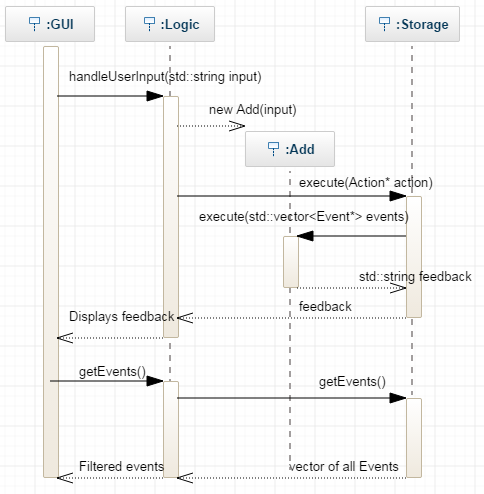
\includegraphics[width=\textwidth]{add_call_diagram}

The logic of the system is explained by the above sequence diagram. The GUI will process the user input into the logic, and it will parse to the controller for the add which later stores it into the storage.

\subsection{Key API}
The only call to the \texttt{Logic} component is made by the \texttt{GUI} when the \texttt{CommandLine::returnPressed()} signal is emitted. The function \texttt{Logic::handleUserInput(std::string)} will then proceed to process the input internally.

\subsection{Controller}

The controller(Logic component) is responsible for creating and executing commands. The user input is received by the controller and passed to the parser. The controller then receives the details of the user command from the parser and performs the action required (add, delete, edit, etc) detailed in the use cases in the appendix.

\begin{center}
\begin{tabular}{|l|r|}
Method                & Return Type \\
create(string input)  & pointer     \\
execute(string input) & pointer    
\end{tabular}
\end{center}

\subsection{Parser}

The parser deciphers user input and creates the relevant command based on the user input. It these sends the command to the controller for execution.

\begin{center}
\begin{tabular}{|l|r|}
Method              & Return Type \\
parse(string input) & pointer    
\end{tabular}
\end{center}

\subparagraph{1} All handlers(add, delete, etc) must use the parse() method and the argument must accept the string parameter.

\subparagraph{2} The parser should not modify the storage. If a task is supposed to be added, the parser should only generate the necessary fields of the task.

\subparagraph{3} All arguments which have an index, the parser must obtain the relevant information of the task which is then returned to the handlers.

\subparagraph{4} The exceptions thrown by the parser should be caught by the associated handler methods.

\subsection{Commands}
BoxIn currently recognizes the following user commands
//add a class diagram here 
\subparagraph{Sort}
Within the Command class, the information will be sorted out so it would be easier to parse out later.

\begin{center}
\begin{tabular}{  lrrl}
\hline
add & edit & delete\\
\hline
undo & view\\
\hline     
\end{tabular}
\end{center}

\newpage

\section{Parsers}
The parsers for BoxIn deal with extracting information out of a user-given string. There are two parsers used in BoxIn - the SimpleParser (for generic items) and the TimeParser, which deals exclusively with times

\subsection{SimpleParser}
The SimpleParser deals more with dates and basic parsing. The following date formats are accepted: \texttt{DDMMYY, YYYYMMDD, YYYY/Jan/DD, monday, tuesday etc, today, tomorrow}.\\

\subparagraph{Type Definitions}
\begin{tabular}{c c}
Type Name & Purpose\\
\hline
InfoType & Determines the information to be extracted\\
DateFormat & Matches the date format to the correct parsing algorithm\\
\end{tabular}

\subparagraph{Private attributes}
\begin{tabular}{c c}
Attribute type & Name\\
\hline
std::map<InfoType, std::string> & keywordMap\\
std::map<std::string, std::string> & monthMap\\
std::map<std::string, boost::date\_time::weekdays> & dayMap\\
\end{tabular}

\subparagraph{Public methods}
\begin{tabular}{c c}
Return Type & Method\\
\hline
std::string & getField(std::string input, InfoType info)\\
void & setupMaps()\\
bool & isKeyword(std::string word)\\
bool & isInteger(std::string text)\\
boost::gregorian::date & convertToDate(std::string date)\\
DateFormat & matchFormat(std::string date)\\
bool & isNumericalFormat(std::string date)\\
bool & isDayOfWeek(std::string day)\\
bool & isToday(std::string day)\\
bool & isTomorrow(std::string day)\\
std::string & removeEscapeChar(std::string word)\\
std::string & removeWhitespace(std::string text)\\
\end{tabular}

\subparagraph{Key API}The \texttt{SimpleParser} implements the following key API to extract data. Many of the functions are used to match dates\\
\begin{tabular}{p{6cm} p{12cm}}
Method & Description\\
\hline
getField() & Retrieves the information matching the InfoType provided by the caller\\
isKeyword() & Returns \texttt{true} if the word given is a keyword\\
removeEscapeChar() & Returns the word removing the escape character \texttt{.}\\
removeWhitespace() & Trims trailing whitespace on a string\\
convertToDate() & Converts a string into a boost::gregorian::date object by matching formats using the other functions. If a match is not found, returns boost::gregorian::not\_a\_date\_time\\
matchFormat() & Returns the format which matches the string it was given. If an appropriate format is not found, returns \texttt{FormatNotRecognised}\\
\end{tabular}

\subsection{TimeParser}
The TimeParser deals in particular with the parsing of times from user strings. The following formats are accepted: \texttt{HHMM, HH:MM}

\subparagraph{Key API}
The TimeParser only implements one key method\\
\begin{tabular}{p{6cm} p{12cm}}
Method & Description\\
\hline
convertToTime() & Converts a string into a boost::posix\_time::ptime object by identifying it by length. Returns boost::date\_time::not\_a\_date\_time
\end{tabular}

\newpage

\section{Storage}
The Storage class keeps both the internal representaion and the json representation of the Event classes. There are 3 major components, discussed below

\subsection{SimpleStorage}
SimpleStorage is the highest level structure of the Storage component of BoxIn. It handles all the interactions with the Logic component.
\subparagraph{Type Definitions}
\begin{tabular}{c c}
Type Name & Purpose\\
\hline
SortCriteria & Determines the sorting method\\
\end{tabular}
\subparagraph{Private attributes}
\begin{tabular}{c c}
Attribute type & Name\\
\hline
std::vector<Event*> & events\\
std::stack<Action*> & actionStack\\
FileStorage & file\\
SortCriteria & criteria \\
\end{tabular}
\subparagraph{Public methods}
\subparagraph{Key API}

\subsection{Event}	 					
The Event class stores data of one Event.
\subsection{FileStorage}


\newpage

\section{Appendix A}

\subsection{Use cases}
\begin{tabular}{l|l}
Name                  & UC01:Add a new task                                                                                                                                                                                                                \\
Description           & To add a new task                                                                                                                                                                                                                  \\
Precondition          & BoxIn is currently running                                                                                                                                                                                                         \\
Basic course of event & \begin{tabular}[c]{@{}l@{}}1. User indicates the event that they want to add (Name, Date, Time, Place)\\and it has to be in this specific order\\ 2. BoxIn will give feedback indicating that the event has been added\end{tabular} \\
Alternative path      & \begin{tabular}[c]{@{}l@{}}1. One of the parameter is missing :\\ \\      1a. BoxIn responds that a parameter is missing and ask the user to try again\end{tabular}                                                                \\
Post Condition        & A new event is added and saved.                                                                                                                                                                                                   
\end{tabular}
\linebreak
\\[1cm]
\begin{tabular}{l|l}

Name                  & UC02: Delete a task                                                                                                                        \\
Description           & To delete an existing task.                                                                                                                                        \\
Pre Condition         & BoxIn is already running.                                                                                                                                          \\
Basic Course of Event & \begin{tabular}[c]{@{}l@{}}1. User types the command to delete an already existing task.\\ 2. The program deletes the task as per the user's command.\end{tabular} \\
Alternative Path      & \begin{tabular}[c]{@{}l@{}}1. If the task does not exist, the program displays the relevant message.\\ 2. Prompts the user to re-enter the command.\end{tabular}   \\
Post Condition        & The task is updated                                                                                                                                               
\end{tabular}
\linebreak
\\[1cm]
\begin{tabular}{l|l}

Name                  & Edit a task                                                                                                                                                                     \\
Description           & To edit an existing task                                                                                                                                                                                      \\
Pre Condition         & BoxIn is already running                                                                                                                                                                                      \\
Basic Course of Event & \begin{tabular}[c]{@{}l@{}}1. User types the command to edit an already existing task and \\specifying the relevant fields to be changed\\ 2. The program edits the task as per the user's command\end{tabular} \\
Alternative Path      & \begin{tabular}[c]{@{}l@{}}1. If the task does not exist, the program displays the relevant message.\\ 2. Prompts the user to re-enter the command.\end{tabular}                                              \\
Post Condition        & The task is updated                                                                                                                                                                                          
\end{tabular}
\linebreak
\\[1cm]
\begin{tabular}{l|l}
Name                  & UC04: Undo action                                                                                                                                   \\
Description           & To undo the previous command                                                                                                                                                \\
Pre Condition         & BoxIn is already running.                                                                                                                                                   \\
Basic Course of Event & 1. User types the command to undo the previous command.                                                                                                                     \\
Alternative Path      & \begin{tabular}[c]{@{}l@{}}1. If the previous action does not exist, the program displays the relevant \\message.\\ 2. Prompts the user to re-enter the command.\end{tabular} \\
Post Condition        & The task is deleted.                                                                                                                                                       
\end{tabular}
\linebreak
\\[1cm]
\begin{tabular}{l|l}

Name                  & UC05: Search task                                                                                                                                          \\
Description           & To search a task                                                                                                                                                                   \\
Pre Condition         & BoxIn is already running.                                                                                                                                                          \\
Basic Course of Event & \begin{tabular}[c]{@{}l@{}}1. User types the command to search for a task.\\ 2. The result is displayed.\end{tabular}                                                              \\
Alternative Path      & \begin{tabular}[c]{@{}l@{}}1. If the syntax does not match, prompts the user to re-enter the command.\\ 2. If the task does not exist, relevant message is displayed.\end{tabular} \\
Post Condition        & The task is undone.                                                                                                                                                               
\end{tabular}
\linebreak
\\[1cm]
\begin{tabular}{l|l}
Name                  & UC06: Sort task                                                                                                  \\
Description           & To sort tasks                                                                                                                            \\
Pre Condition         & BoxIn is already running.                                                                                                                \\
Basic Course of Event & \begin{tabular}[c]{@{}l@{}}1. User types the command to sort the tasks.\\ 2. The program displays the task in sorted order.\end{tabular} \\
Alternative Path        & 1. Sort criteria is not specified and tasks are sorted using the default order.             	                                                                                                                       \\
Post Condition        & -                                                                                                                                       
\end{tabular}
\linebreak
\\[1cm]
\begin{tabular}{l|l}

Name                  & UC07: Display task                                                                                      \\
Description           & To display a task                                                                                                               \\
Pre Condition         & BoxIn is already running.                                                                                                       \\
Basic Course of Event & \begin{tabular}[c]{@{}l@{}}1. User types the command to display the task.\\ 2. The program displays the task.\end{tabular}      \\
Alternative Path      & \begin{tabular}[c]{@{}l@{}}1. The relevant task does not exist.\\ 2. Program prompts the user to re-enter command.\end{tabular} \\
Post Condition        & -                                                                                                                              
\end{tabular}
\newpage

\section{Appendix B: Setting up}
To set up, you will need Windows Operating System, VS2012, Boost, and Git.
\subsection{Qt 5.3.1}
The Visual Studio plugin for Qt. You can find it at http://qt-project.org/downloads. 
Scroll to the bottom of the page and look for qt-vs-addin-1.2.3-opensource.exe. 
Then open Visual Studio. The top bar should show QT5 -> QT Options. Make 
sure that the correct version of QT is selected. 
Install Qt to C:/Qt
\subsection{Boost}
Boost libraries - version 1.57, vc2012 (vc11.0), 32 bit. You can find it at\\
\url{http://tinyurl.com/BoxInDevBoost}\\ and install to \texttt{C:/Boost}
\subsection{3.Visual Studio plugin}
The Visual Studio plugin for Qt. You can find it at http://qt-project.org/downloads. 
Scroll to the bottom of the page and look for qt-vs-addin-1.2.3-opensource.exe. 
Then open Visual Studio. The top bar should show QT5 -> QT Options. Make 
sure that the correct version of QT is selected. 
\subsection{4.Git}
You can download git from Github.com and register as a member, then clone the software and open the file and it should work out!

\section{Appendix C: Testing Instructions}
Both unit tests and system tests are held in the same project file \texttt{(UnitTest)} and all code is contained in \texttt{unittest.cpp}, with headers in \texttt{unittest.h}
\subparagraph{Setting up}
Change the directory of the include directory to match that of the project directory
\subparagraph{Prerequisites to testing}
To create any unit test that would include any GUI components, it is necessary to first start a QApplication. Refer to the following code example. \texttt{foo} is a defined function used to create the integer reference, but has no further use. The application need not be used further.\\
\texttt{int\& argc = foo();\\
char** argv;\\
QApplication app(argc, argv);
}
\subparagraph{Testing policy}
All newly added code should come together with a series of unit tests to prove it works for both the general and the borderline cases. Also, before committing any new code, it must clear all system level tests.

\subparagraph{Note on Qt}
It is possible to get the system to run events by using the emit function to generate te signals that normally would be generated from user activity

\newpage
\section{Appendix D: Full Class Diagram}
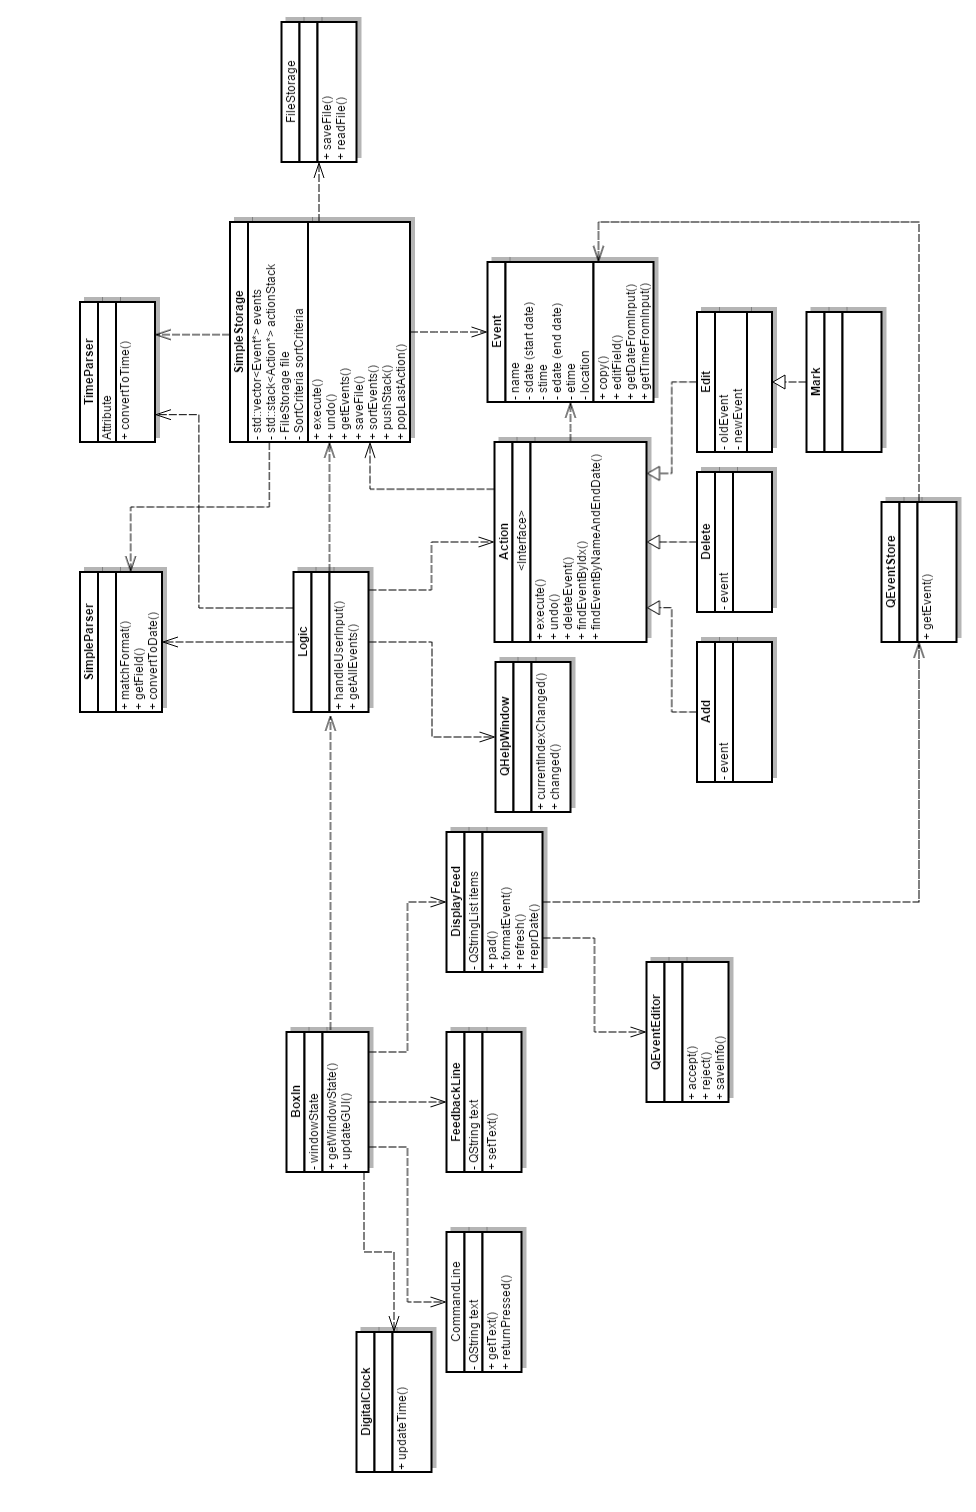
\includegraphics[width=\textwidth, height=\textheight - 2cm]{class_diagram}

\end{document}